\begin{figure}[t]
\centering
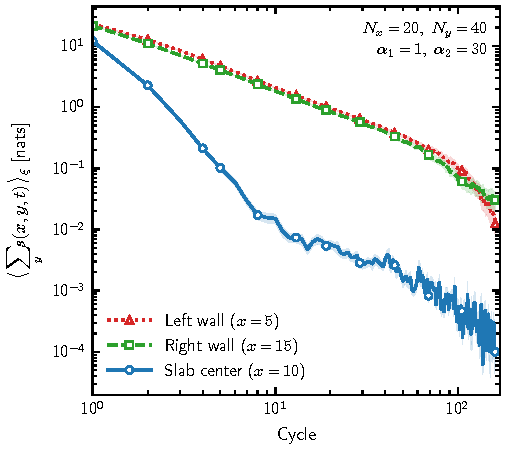
\includegraphics[width=\columnwidth]{hard_n20x40_wall_center_entropy_loglog.pdf}
\caption{Spatially resolved purification for a $20\times40$ hard-wall system,
$\alpha_1=1$ and $\alpha_2=30$. The entropy contour is summed along $y$ at
the left wall ($x=5$), right wall ($x=15$), and slab center ($x=10$),
then averaged over 100 independent trajectories; bands show ordinary
trajectory SEM. The active slab starts maximally mixed after Born-conditioned
exterior preparation, with slab-only measurements, perfect correction,
$n_{\rm shell}=1$, and raster-$y$ ordering. Raw cycles $1$--$160$ are shown
on logarithmic axes; cycle zero is omitted. No fit is imposed.}
\label{fig:hard-n20x40-wall-center-purification}
\end{figure}
